\chapter{Approches Proposés}
\section{Introduction}
\noindent
Dans cette section en va explorer les différentes solutions potentielles et les différents approches qu'on a pris pour améliorer la recherche dans notre projet. Nous aborderons chacune des technologies utilisés en expliquant leurs fonctions principales, leurs utilisations courantes et leurs avantages. Nous discuterons également de l'importance de ces outils dans le domaine de l'analyse de texte et du traitement du langage naturel. En comprenant ces différentes approches, nous serons en mesure d'explorer en détail leurs fonctionnalités spécifiques et leur pertinence pour notre projet de PFE.

\section{Les solutions possibles}
\noindent
Dans cette section on va explorer les solutions potentielles qu'on peut adopter pour notre projet tel que les différentes techniques de recherches et les bases de donnèes qu'on peut utiliser. 

\subsection{Recherche Régulière}
\noindent
Nous aurions pu utiliser la recherche régulière simplement en faisant correspondre le terme de recherche avec les phrases disponibles dans notre base de données SQL déja existante via des requêtes SQL beaucoup plus optimisés et rapides. Avec cette approche, il y a moins de travail et complexité, mais des résultats beaucoup moins précis.

\subsection{Utilisaton d'une base de donnèes SQL altèrnatif et performante}
\noindent
Nous aurions pu utiliser une différente base de donnèes SQL plus optimisé et performante comme Cassandra pour l'optimisation de vitesse de recherche et la prècision des resultats renvoyès. Avec cette approche la migration des donnèes existantes va être beaucoup plus complexe aussi que l'intègration de cette base de donnèes dans notre application. Mais les rèsultate vont être plus prècis et rapide, mais il reste la limitation la plus importante, qui est la recherche en Arabe avec le dialecte Tunisien, et l'Arabe Traditionnelle. Pour cette raison on a dècidè de prendre l'approche d'Elasticsearch avec le recherche vectorielle qui sont dans les sections ci-dessous.

\section{Choix d'approche de Recherche Vectorielle}
\noindent
En raison des défauts des autres solutions que nous avons mentionnées dans la section précédente, nous avons décidé d'opter pour l'approche de recherche vectorielle, que nous expliquerons plus en détail dans la section suivante.

\begin{figure}[H]
\centering
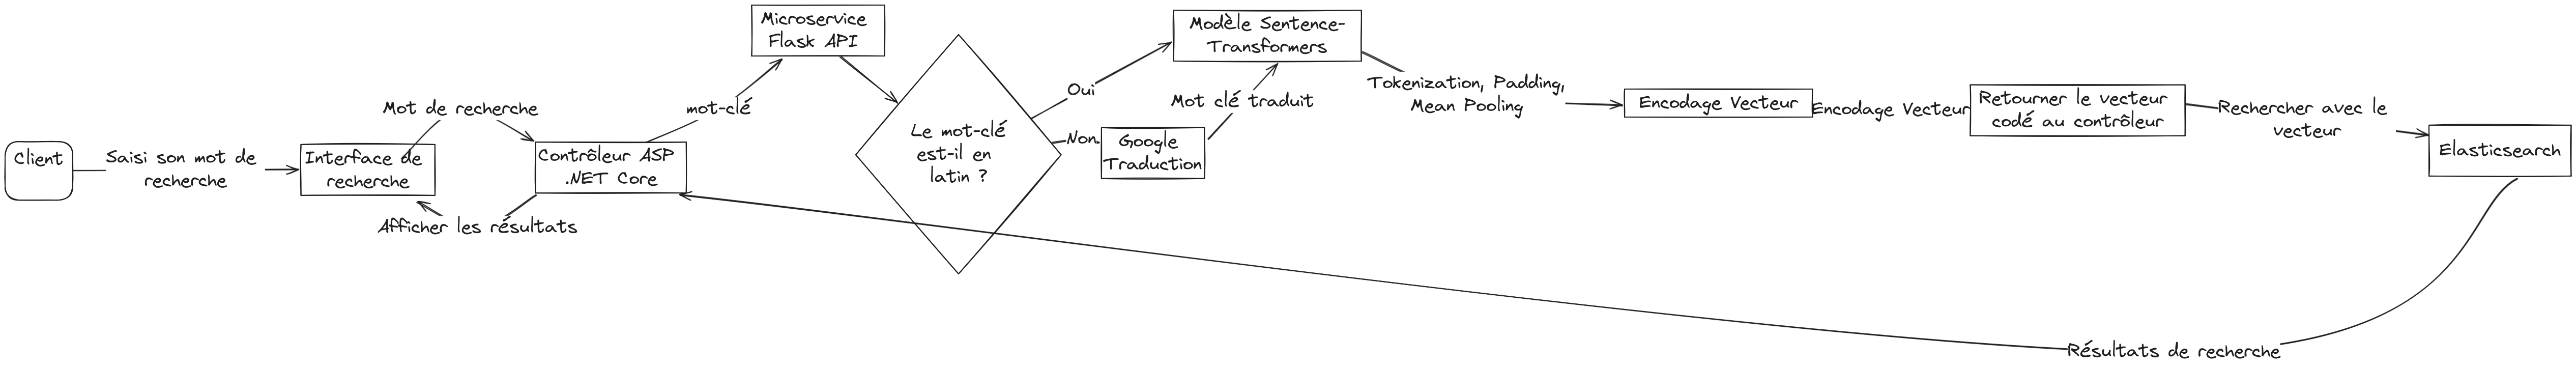
\includegraphics[width=1\textwidth]{logos/generalisedprocess.png}
\caption{Présentation du processus de recherche avec recherche vectorielle}
\label{fig:generalisedprocess}
\end{figure}

\newpage
\noindent
Comme la figure ~\ref{fig:generalisedprocess} montre, d'abord le client va saisir son terme de recherche (mot clé) qui est ensuite envoyé à notre contrôleur ASP .NET Core, qui ensuite envoie cette mot ou phrase à notre microservice en Flask qui contient notre modéle Sentence-Transformers(all-mpnet-base-v2) dans notre cas, qui ensuite verifient si le mot est en Français, si c'est le cas, en fait l'encodage du phrase directe, sinon, en la traduit soit en utilisant Google Traduction si la phrase est en Arabe Traditionnelle, soit en utilisant notre dictionnaire propre des mots du dialecte Tunsienne et aprés faire l'encodage, enfin, le vecteur est renvoyé au contrôleur, qui l'utilise pour faire le recherche vectorielle dans Elasticsearch, et renvoyer les résultats, qui sont les produits dans notre cas.


\section{Recherche Vectorielle}
\noindent
La recherche vectorielle est une approche de la récupération des informations qui prend en charge l’indexation et l’exécution des requêtes sur des représentations numériques du contenu. Étant donné que le contenu est numérique plutôt que texte brut, la correspondance est basée sur des vecteurs qui sont les plus similaires au vecteur de requête, ce qui permet la correspondance entre :
\begin{itemize}
    \item La ressemblance sémantique ou conceptuelle (« chien » et « canine », conceptuellement similaire mais linguistiquement distincte)
    
    \item contenu multilingue (« dog » en anglais et « chien » en Français)
\end{itemize}

\noindent
Pour calculer cette similarité Il y a plusieurs approches de calcul, la plus significante, précis et populaire c'est la similarité cosinus qui utilise cette formule mathématique:
\[\cos(\theta) = \frac{\mathbf{A} \cdot \mathbf{B}}{\|\mathbf{A}\|\|\mathbf{B}\|} = \frac{\sum_{i=1}^{n} A_i B_i}{\sqrt{\sum_{i=1}^{n} A_i^2} \sqrt{\sum_{i=1}^{n} B_i^2}}
\]
Soit $A$ et $B$ deux vecteurs de n'importe quelles dimensions, la similarité cosinus mesure l'angle entre deux vecteurs. Plus l'angle est petit, plus les vecteurs sont similaires, le cosinus de leur angle $\theta$ s'obtient en prenant leur produit scalaire divisé par le produit de leurs normes. Le valeur de cette angle est compris entire [-1, 1], la valeur de -1 indique des vecteurs opposés, la valeur de 0 des vecteurs indépendants (orthogonaux) et la valeur de 1 des vecteurs colinéaires de coefficient positif. Plus que cette valeur s'approche de 1, le plus que les deux vecteurs sont similaires.

\begin{figure}[H]
\centering
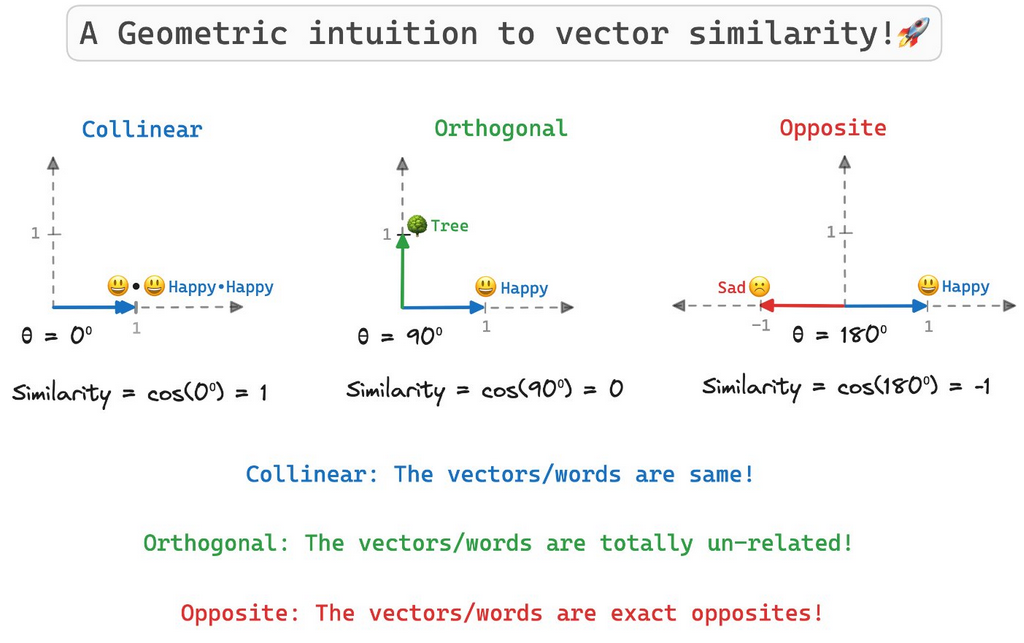
\includegraphics[width=1\textwidth]{logos/cosine.png}
\caption{Présentation du similarité cosinus}
\label{fig:cosine}
\end{figure}

\section{Elasticsearch}
\noindent
Elasticsearch est un outil d'analyse de donnèes distribuès open source et hautement èvolutif. Il est conçu pour stocker, rechercher et analyser et rechercher de grands volumes de données de manière rapide et efficace en utilisant des diffèrents mèthodes comme Knn Search.
Il utilise une structure de données de type index inversé pour indexer et rechercher rapidement des documents. Il prend en charge une variété de types de données, notamment le texte, les nombres, les dates, et les vecteurs par exemple le type dense vector. Avec tout sa, Elasticsearch facilite et optimise la recherche sémantique(vectorielle) en utilisant des indices inversés qui nous permet de stocker des données de type dense vector (vecteur), qui sont extrêmement efficaces pour la recherche de texte complet. Au lieu de parcourir chaque document et de vérifier la correspondance avec les termes de la requête, Elasticsearch utilise cet indice inversé pour trouver rapidement les documents contenant les termes de recherche. Cela accélère considérablement le processus de recherche, car l'indice fonctionne comme un système de référence rapide.

\section{Utilisation d'un modéle Sentence-Transformers}
\noindent
Notre modéle de choix est un modéle appelé << all-mpnet-base-v2 >> qui est basé sur le modèle mpnet-base de Microsoft, et puisqu'il est déja pré-entraînée pour comprendre la langue Française. Il sert a convertir des des phrases et des paragraphes en vecteurs sémantiques de 768 dimensions dans un espace vectoriel, avec une limite des paragraphes de 384 mots au maximum. Il est spécifiquement affiné pour établir des correspondances sémantiques précises entre les phrases en les plaçant dans un espace où la similarité cosinus peut être calculée efficacement pour des tâches comme la recherche sémantique, et la mesure de la similarité des phrases. \\
\citetitle{pinecone:mpnet} (\cite{pinecone:mpnet})

\subsection{Comment le modéle intérpréte les phrases?}
\noindent
Pour interpréter les phrases, le modéle est besoin d'un << Tokenizer >> puisqu'il ne peux pas comprendre du texte, on doit convertir chaque phrase en une représentation numérique. Le processus est appelé la << tokenisation >> qui est le processus de conversion d'une séquence de caractères en une séquence de jetons(tokens). En PNL, un jeton(token) représente généralement un mot, mais il peut également représenter des sous-mots, des caractères ou d'autres unités, selon le tokeniseur. Ce processus est nécessaire car notre modèle ne peux pas comprendre le texte brut. Au lieu de cela, il travail avec des représentations numériques de jetons. La figure ~\ref{fig:paddingexplanation} présente le processus de tokenisation.

\begin{figure}[H]
\centering
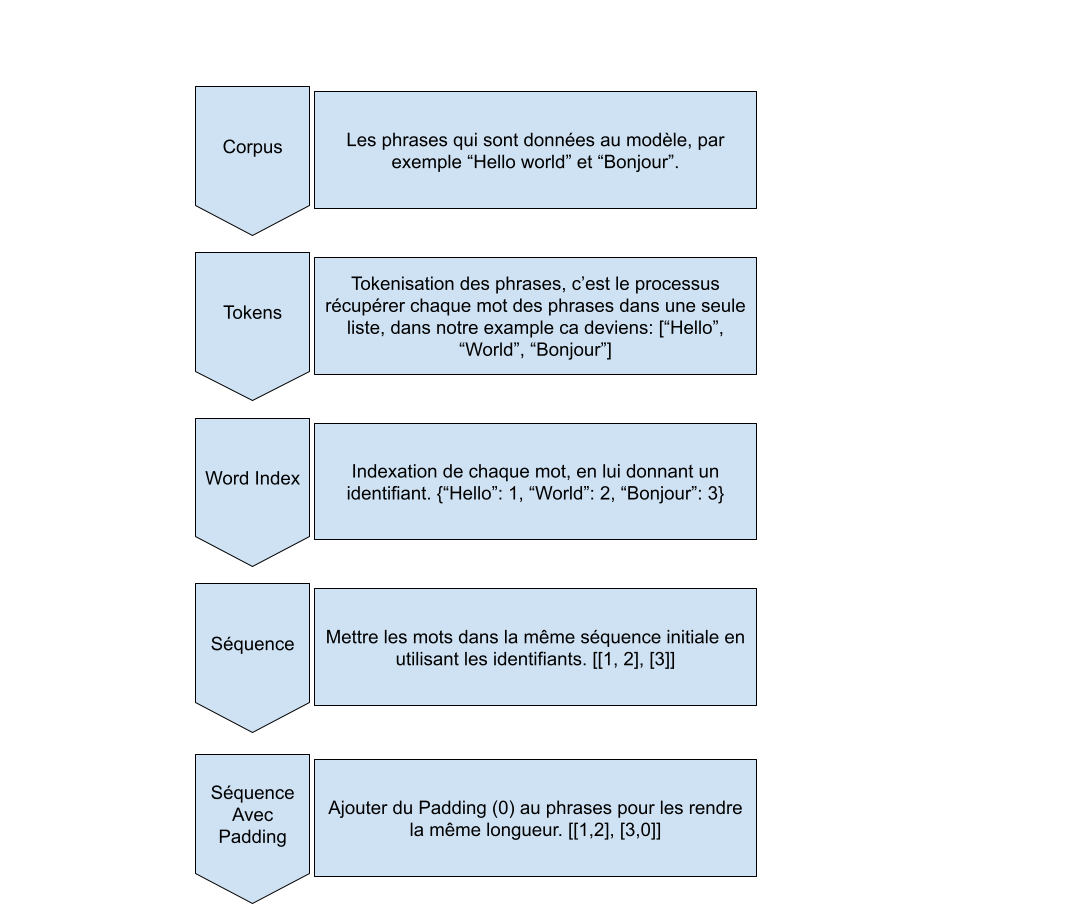
\includegraphics[width=1\textwidth]{logos/paddingexplanation.png}
\caption{Presentation du processus de tokenisation}
\label{fig:paddingexplanation}
\end{figure}

\noindent
La figure ~\ref{fig:padding} présente un exemple du processus de tokenisation.

\begin{figure}[H]
\centering
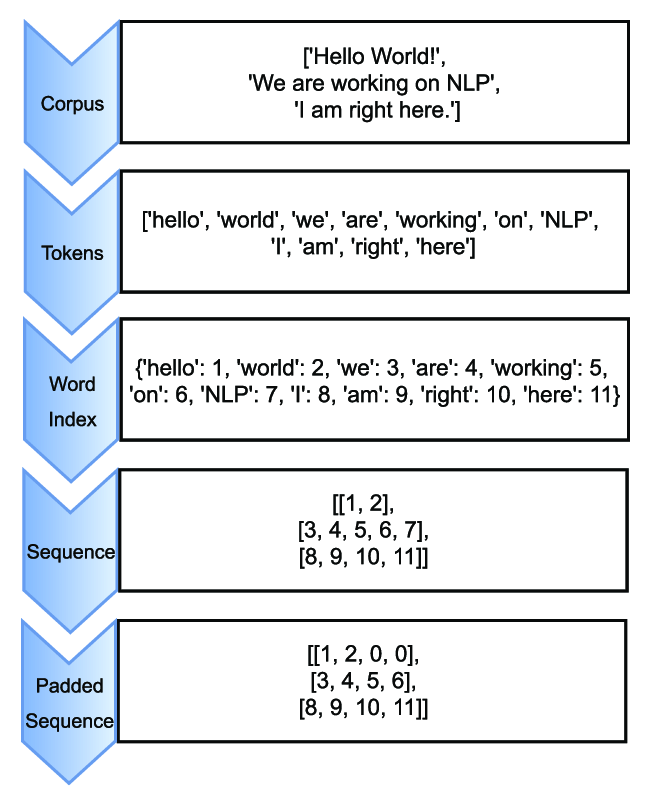
\includegraphics[width=1\textwidth]{logos/padding.png}
\caption{Exemple du processus de tokenisation}
\label{fig:padding}
\end{figure}

\newpage
\noindent
{\small\textbf{\textit{a. Padding }}}\mbox{}\\
Le remplissage(padding) est appliqué pour garantir que toutes les séquences d'un lot ont la même longueur, ce qui est une exigence pour de nombreuses architectures de réseaux neuronaux. Des jetons de remplissage sont ajoutés à la fin de la séquence pour étendre sa longueur jusqu'à un maximum prédéfini, qui est de 384 dans notre cas.

\noindent
{\small\textbf{\textit{b. Attention Mask (Masque d'attention) }}}\mbox{}\\
C'est simplement un masque qui fait la différence entre le contenu et les jetons de remplissage.

\noindent
{\small\textbf{\textit{c. Mean Pooling (Regroupement des moyennes) }}}\mbox{}\\
C'est un processus qui calcule efficacement la moyenne de la sequence obtenu aprés le padding tout en ignorant les jetons de remplissage (padding tokens) qui ont une valeur de 0, ce qui donne un seul vecteur d'intégration qui représente la phrase entière.
Ce processus ne prend en compte que les jetons sans remplissage dans la phrase, en utilisant un masque d'attention. Le masque d'attention a la même longueur que la séquence de jetons, « 1 » indiquant les jetons sans remplissage et « 0 » pour les jetons de remplissage. Cela garantit que l'incorporation de phrase résultante est calculée uniquement à partir du contenu significatif de la séquence. La figure ~\ref{fig:meanpooling} présente ce processus.

\begin{figure}[H]
\centering
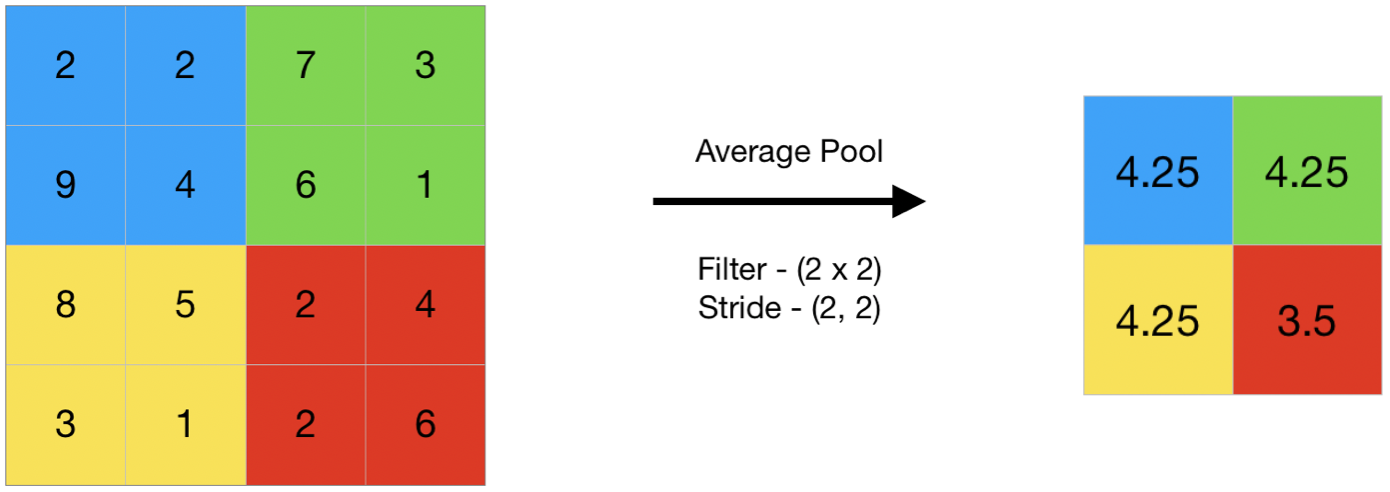
\includegraphics[width=1\textwidth]{logos/mean_pooling.png}
\caption{Présentation du processus de Mean Pooling}
\label{fig:meanpooling}
\end{figure}

\subsection{Pourquoi utiliser Mean Pooling plutôt qu'un autre type de pooling?}
\noindent
Puisque notre modéle génère un vecteur pour chaque token aprés les étapes précédentes, le mean pooling consiste à prendre la moyenne de ces vecteurs sur tous les tokens, ce qui résulte en un unique vecteur qui est censé capturer l'essence sémantique de l'ensemble de la phrase, et donner importance à tous les mots de phrase, tous en nous permettant de prendre et interpréter le contexte de toute la phrase. Il existe deux autres types do pooling qu'on a testé sans obtenir de résultats aussi bons:

\noindent
{\small\textbf{\textit{a. Max Pooling }}}\mbox{}\\
Ce processus consiste à prendre la valeur maximum de ces vecteurs sur tous les tokens au lieu de la moyenne. La probléme avec cette stratégie est ce que elle peut donner plus importance à une mot ou phrase plus que les autres et alterner les résultats de manière négative, ce qui entraîne moins de précision. Par exemple, si un personne cherche pour un << T-shirt bleu >>, avec le max pooling, le mot << bleu >> peut avoir plus d'importance que t-shirt, donc il peut retourner tous les produits bleus, au lieu des t-shirts. La figure ~\ref{fig:maxpooling} présente ce processus. 

\begin{figure}[H]
\centering
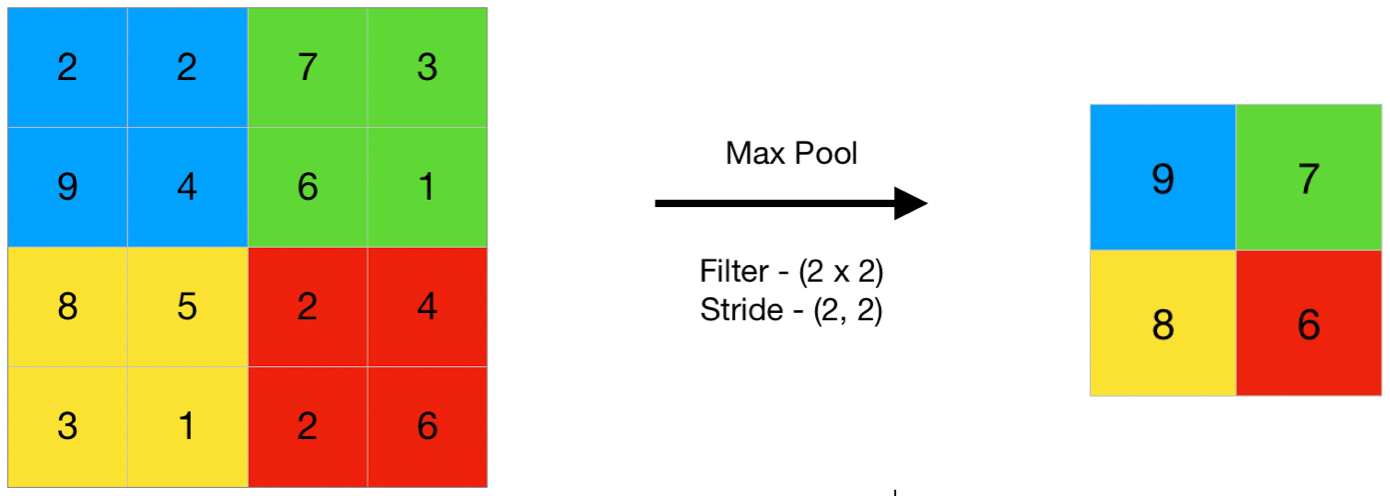
\includegraphics[width=1\textwidth]{logos/max_pooling.png}
\caption{Présentation du processus de Max Pooling}
\label{fig:maxpooling}
\end{figure}

\newpage
\noindent
{\small\textbf{\textit{b. Min Pooling }}}\mbox{}\\
Ce processus consiste à prendre la valeur minimum de ces vecteurs sur tous les tokens au lieu de la moyenne. La probléme avec cette stratégie est ce que elle peut donner moins importance à une mot ou phrase clé moins que les autres et alterner les résultats de manière négative, ce qui aussi entraîne moins de précision. Prenant le même exemple précédent, si un personne cherche pour un << T-shirt bleu >>, avec le min pooling, le mot << bleu >> peut avoir moins d'importance que t-shirt, donc il peut retourner tous les t-shirts sauf les bleus. La figure ~\ref{fig:minpooling} présente ce processus. 

\begin{figure}[H]
\centering
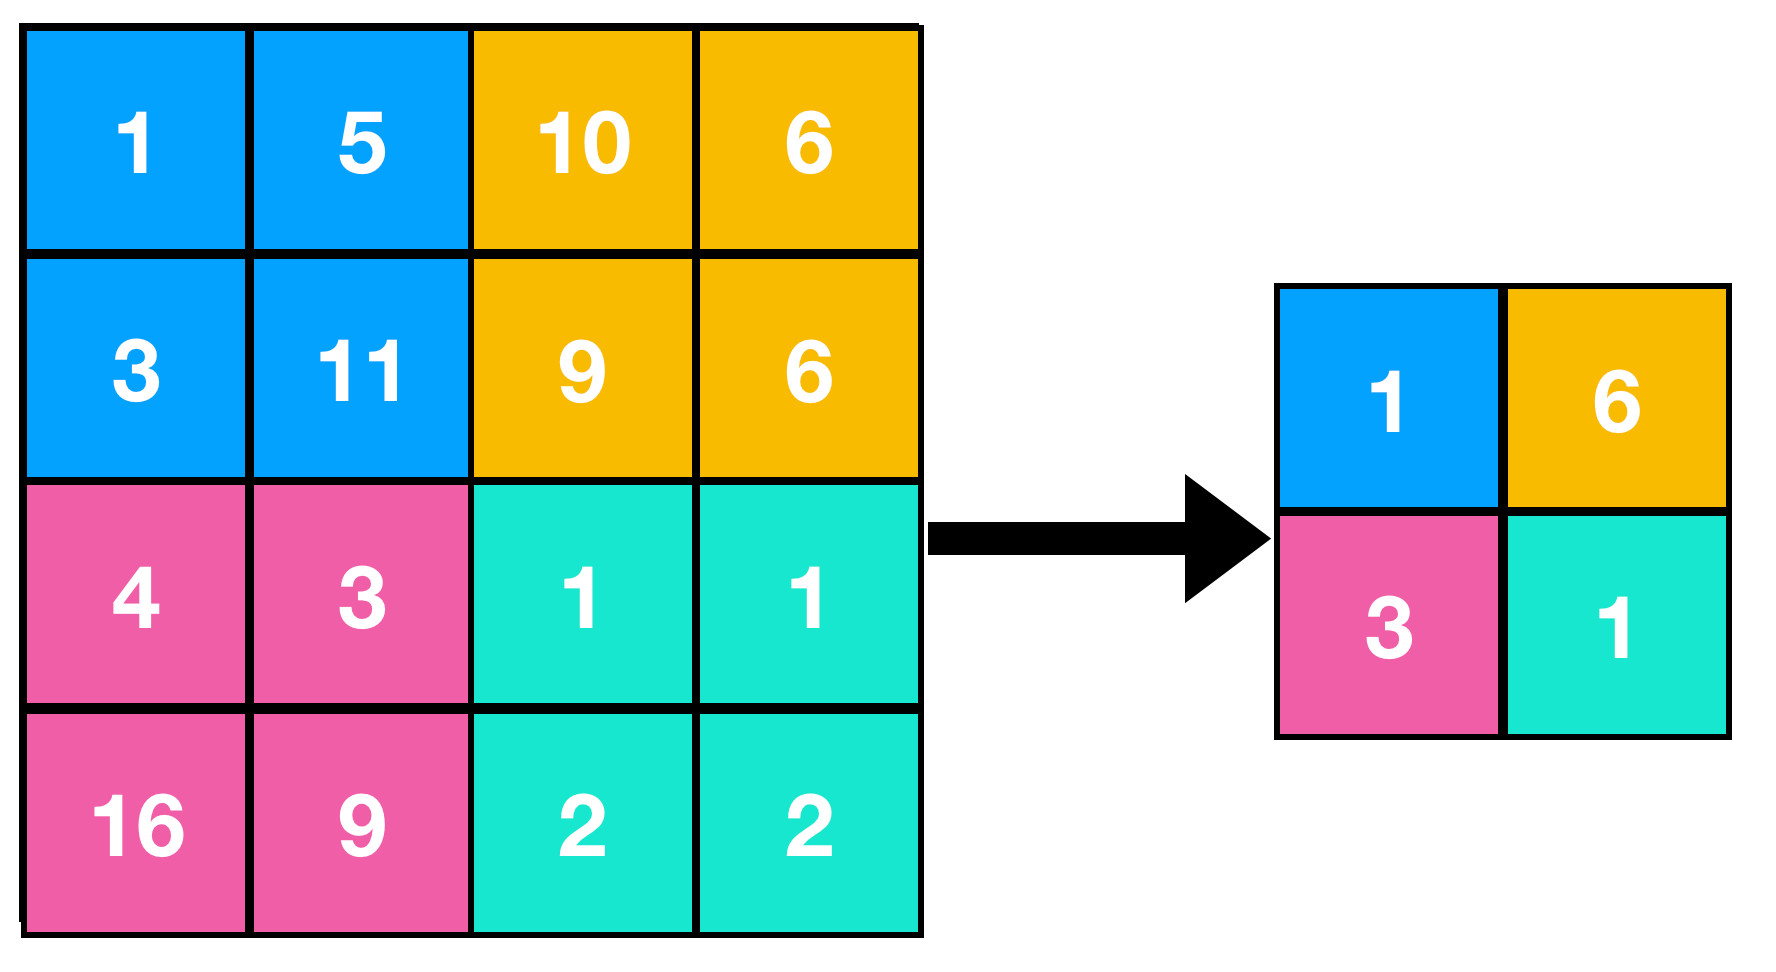
\includegraphics[width=1\textwidth]{logos/min_pooling.png}
\caption{Présentation du processus de Min Pooling}
\label{fig:minpooling}
\end{figure}


\section{Conclusion}
\noindent
Dans cette section on a presenté et expliqué les approches qu'on a décidé de prendre ainsi que les technologies qu'on a utilisé et leurs importance, pertinence et les benéfices qu'ils apportent a notre projet tels que le Recherche Vectorielle, l'Elasticsearch et le modéle sentence-transformers.